\documentclass[conference]{IEEEtran}
\IEEEoverridecommandlockouts

\usepackage[T5,T1]{fontenc}
\usepackage[utf8]{inputenc}
\usepackage[vietnamese,english]{babel}
\usepackage{cite}
\usepackage{amsmath,amssymb}
\usepackage{graphicx}
\usepackage{booktabs}
\usepackage{multirow}
\usepackage{array}
\usepackage{xcolor}
\usepackage[hidelinks]{hyperref}

\newcommand{\vn}[1]{\foreignlanguage{vietnamese}{#1}}
\newcommand{\ci}[2]{\scriptsize[#1,\,#2]}

\begin{document}

\title{Geography-Aware Province-Level Vietnamese Dialect Identification with Frozen Self-Supervised Speech Representations}

\author{\IEEEauthorblockN{Tho Dang}
\IEEEauthorblockA{\textit{University of Information Technology, VNU-HCM}\\
Ho Chi Minh City, Vietnam\\
Student ID: 24521715}}

\maketitle

\begin{abstract}
We study province-level Vietnamese dialect identification on ViMD, a 102-hour corpus covering all 63 provinces. Instead of fine-tuning, we keep self-supervised speech encoders frozen and train a light head over a learned weighted sum of their layers. Our best system fuses XLS-R and PhoWhisper representations and reaches 64.6\% accuracy and 0.637 macro-F1 on the official test set, against 0.411 macro-F1 for the best fine-tuned model reported with the dataset. We also propose Geo-aware Label Smoothing (Geo-LS), which spreads the smoothing mass to geographically close provinces. On the fused model, Geo-LS lowers the mean distance between the true and predicted province by 8.2\,km (95\% CI 1.4 to 14.6) at no significant cost in accuracy, and raises region accuracy to 94.4\%. Controlled experiments show that the model does not rely on spoken place names or on recording-channel spectra alone. Full fine-tuning, LP-FT and more complex temporal architectures did not beat the frozen-feature approach in this low-resource setting, with about 240 training utterances per province.
\end{abstract}

\begin{IEEEkeywords}
dialect identification, Vietnamese, self-supervised learning, XLS-R, Whisper, label smoothing, geographic distance
\end{IEEEkeywords}

%======================================================================
\section{Introduction}
Vietnamese is usually described with three dialect regions, Northern, Central and Southern, but pronunciation also varies from province to province. Knowing a speaker's dialect helps speech recognition, speaker profiling and sociolinguistic research. The ViMD corpus~\cite{vimd} made the fine-grained task measurable by labelling speech from all 63 provinces. Its baselines fine-tune wav2vec~2.0 and Whisper models and reach at most 0.411 macro-F1.

The task has two properties that standard classification ignores. First, the classes have a geography: confusing \vn{Hà Nội} with \vn{Hà Nam} is a much smaller error than confusing it with \vn{Cà Mau}. Second, a province label can be predicted from cues that are not dialect at all, such as place names spoken in the recording or the acoustic signature of the local broadcaster that recorded it. A useful study has to measure both.

This paper asks four research questions:
\begin{enumerate}
\item[\textbf{RQ1}] How far can frozen self-supervised speech representations go on 63-way dialect identification?
\item[\textbf{RQ2}] Does the model hear accent, or does it exploit spoken content and recording channel?
\item[\textbf{RQ3}] Can a training objective that knows the map make errors geographically closer without losing accuracy?
\item[\textbf{RQ4}] Do fine-tuning or temporal architectures add anything over pooled frozen features at this data size?
\end{enumerate}

Our contributions are:
\begin{itemize}
\item A frozen-encoder pipeline with a learned layer-weighted head that reaches 64.6\% accuracy and 0.637 macro-F1 on the ViMD test set, about 0.23 macro-F1 above the published baselines.
\item A set of confound controls, including text-only, spectrum-only and place-name-free evaluations, showing that most of the accuracy comes from accent.
\item Geo-aware Label Smoothing (Geo-LS), a one-line change to the training target that consistently reduces geographic error by 8 to 19\,km across settings.
\item Negative results with diagnostics for full fine-tuning, LP-FT and frame-level CNN and Transformer heads, plus a layer-wise analysis showing that dialect information peaks in the middle layers of both XLS-R and PhoWhisper.
\end{itemize}

%======================================================================
\section{Related Work}
\textit{Vietnamese dialect identification.} Earlier Vietnamese work mostly separated the three regional dialects. ViMD~\cite{vimd} introduced province-level labels for 63 provinces and benchmarked fine-tuned wav2vec~2.0, XLS-R, Whisper and PhoWhisper models. PhoWhisper-base was best with 0.411 macro-F1, and XLS-R-300m reached 0.373. The authors also found that geography influences which dialects are confused, which motivates our distance-aware objective.

\textit{Self-supervised speech representations.} wav2vec~2.0~\cite{wav2vec2} and its multilingual version XLS-R~\cite{xlsr} learn speech representations from unlabelled audio. Whisper~\cite{whisper} is trained with weak supervision for transcription; PhoWhisper~\cite{phowhisper} adapts it to Vietnamese. The SUPERB benchmark~\cite{superb} evaluates such models frozen, with a learned weighted sum of layers and a light downstream head; we follow this protocol. Layer-wise studies~\cite{pasad} show that different layers encode acoustic, phonetic and lexical information, so the best layer depends on the task.

\textit{Pooling and temporal architectures.} For speaker and language recognition, attentive statistics pooling~\cite{asp} and ECAPA-TDNN~\cite{ecapa} are standard ways to summarise frame-level features. We adapt both as heads over frozen frames.

\textit{Fine-tuning versus probing.} Kumar et al.~\cite{lpft} showed that fine-tuning a pretrained model with a randomly initialised head can distort its features, and proposed LP-FT: train the head first, then fine-tune. We test both strategies.

\textit{Distance-aware objectives.} Label smoothing~\cite{inception,muller} replaces one-hot targets with a mixture of the true label and a uniform distribution. Soft ordinal labels (SORD)~\cite{sord} build targets from a distance between classes, and hierarchy-aware losses~\cite{bettermistakes} aim to make ``better mistakes''. Geo-LS combines the two ideas: it keeps label smoothing's fixed mass on the true class and distributes only the smoothed mass by geographic distance.

%======================================================================
\section{Dataset}
We use ViMD~\cite{vimd} with its official speaker-disjoint splits. Table~\ref{tab:data} summarises the statistics we measured on the released data.

\begin{table}[t]
\centering
\caption{ViMD Statistics}
\label{tab:data}
\begin{tabular}{@{}ll@{}}
\toprule
Property & Value \\
\midrule
Provinces (classes) & 63 (pre-2025 boundaries) \\
Regions & North 25, Central 19, South 19 \\
Utterances & 18,949 \\
\quad train / valid / test & 15,023 / 1,900 / 2,026 \\
Audio & 102.56\,h, mean 19.5\,s / utt. \\
Speakers & 12,953 (88--309 per province) \\
Utterances per province & 263--363 (median 303) \\
Chance accuracy & 1.6\% \\
\bottomrule
\end{tabular}
\end{table}

\textit{Preprocessing.} All audio was resampled to 16\,kHz mono and stored as FLAC. Two speakers appear in both the validation and test sets; we removed their validation utterances, leaving 1,898 validation utterances. The test set is untouched, so our numbers are comparable with the original paper. Most speakers contribute only one or two utterances (about 1.5 on average).

\textit{Geography.} Each province is represented by the coordinates of its capital city, and distances between provinces are great-circle (haversine) distances. The median distance from a province to its nearest neighbour is 44\,km and the maximum is 113\,km. Coordinates are approximate to about 5\,km, which is small compared with these distances.

\textit{Transcripts.} Each utterance comes with a transcript. We use transcripts only for text-only control baselines and to detect spoken place names, never as input to the main model. Many recordings appear to come from local news and public-affairs programmes: the most province-specific words in the transcripts are place names and local topics.

%======================================================================
\section{Methodology}
Our system keeps pretrained speech encoders frozen and trains only a small head: (i)~encode the waveform with a frozen encoder and keep the hidden states of every layer; (ii)~mean-pool each layer over time, using only non-padded frames; (iii)~standardise each layer with training-set statistics and combine the layers with learned softmax weights; (iv)~classify the 63 provinces with a two-layer MLP (512 hidden units, GELU, dropout 0.3).

\subsection{Frozen Backbones}
\textit{XLS-R.} We use wav2vec2-xls-r-300m~\cite{xlsr} (24 Transformer layers, 1,024 dimensions). Probing showed that dialect information peaks around layer~5, so we keep the embedding output and layers 1 to 12 (13 states) and drop the rest. Long utterances are cut into 12-second windows; the pooled features of each window are averaged, weighted by frame count, over up to 60 seconds of audio.

\textit{PhoWhisper.} We use the encoder of PhoWhisper-large~\cite{phowhisper} (32 layers, 1,280 dimensions), a Whisper model fine-tuned for Vietnamese ASR. Whisper always receives 30 seconds of padded log-mel input, so we pool only over frames that correspond to real audio. We keep all 33 states.

\textit{Fusion.} For two backbones, each gets its own layer weights and standardisation; the two pooled vectors are concatenated (2,304 dimensions) before the MLP.

\subsection{Layer-Weighted Pooling}
For layer $l$ with pooled vector $\mathbf{h}_l$, training mean $\boldsymbol{\mu}_l$ and standard deviation $\boldsymbol{\sigma}_l$, the utterance representation is
\begin{equation}
\mathbf{z} = \sum_{l=0}^{L} \frac{\exp(w_l)}{\sum_{k=0}^{L}\exp(w_k)} \cdot \frac{\mathbf{h}_l - \boldsymbol{\mu}_l}{\boldsymbol{\sigma}_l}.
\label{eq:wsum}
\end{equation}
The weights $w$ are learned jointly with the MLP, as in SUPERB~\cite{superb}. Because standardisation and mean-pooling are both linear, features can be pooled once and cached, so each head trains in seconds.

\subsection{Geo-Aware Label Smoothing (Geo-LS)}
Standard label smoothing gives the true province a mass of $1-\varepsilon$ and spreads $\varepsilon$ uniformly over all provinces. Geo-LS keeps $1-\varepsilon$ on the true province but spreads $\varepsilon$ over the other provinces in proportion to their geographic closeness. For true province $i$ and distance $d(i,j)$ in kilometres,
\begin{equation}
q_i(j) =
\begin{cases}
1-\varepsilon, & j = i,\\[2pt]
\varepsilon\,\dfrac{\exp\!\left(-d(i,j)/\tau\right)}{\sum_{k\neq i}\exp\!\left(-d(i,k)/\tau\right)}, & j \neq i.
\end{cases}
\label{eq:geols}
\end{equation}
The model is trained with cross-entropy against $q_i$. We select $\varepsilon$ and $\tau$ on the validation set from $\varepsilon \in \{0.1, 0.2, 0.3\}$ and $\tau \in \{25, 50, 100, 200\}$\,km; the chosen setting is $\varepsilon = 0.3$, $\tau = 200$\,km.

The design responds to a failure of SORD-style targets~\cite{sord}, where all the mass follows the distance kernel. Neighbouring provinces are only about 44\,km apart, so a kernel with $\tau = 50$\,km leaves less than half of the target mass on the true class, and accuracy drops sharply (Section~\ref{sec:obj}). Geo-LS fixes the mass on the true class independently of $\tau$.

\subsection{Frame-Level Architectures}
To test whether temporal patterns such as tone contours add information beyond mean-pooled features, we extract frame-level features (fixed layer weights, 25 frames per second) and train five heads on them: (a)~mean pooling + MLP (control); (b)~mean and standard deviation pooling + MLP; (c)~attentive statistics pooling (ASP)~\cite{asp}; (d)~an ECAPA-style head~\cite{ecapa} with three dilated Conv1D blocks with squeeze-excitation, followed by ASP (2.5\,M parameters); (e)~a two-layer Transformer encoder (4 heads, model dimension 256) followed by ASP (1.6\,M parameters).

\subsection{Fine-Tuning}
We also fine-tune XLS-R end to end, with the convolutional feature encoder frozen and SpecAugment-style time masking~\cite{specaugment} ($p = 0.05$). Variant~1 fine-tunes all 24 layers with a randomly initialised head for 6 epochs on 6-second random crops (encoder learning rate $3\times10^{-5}$, head $10^{-3}$). Variant~2 applies LP-FT~\cite{lpft} to the 12-layer encoder: the head is first trained on frozen features, then the whole model is fine-tuned for 12 epochs with a cosine schedule (encoder $2\times10^{-5}$, head $2\times10^{-4}$).

%======================================================================
\section{Experimental Setup}
\textit{Training.} Heads are trained with AdamW (learning rate $10^{-3}$, weight decay $10^{-3}$, batch 256) for up to 80 epochs, with early stopping on validation accuracy (patience 10). Every configuration is run with 3 seeds. Hyperparameters and model choices are selected on the validation set only; the test set is used once per configuration.

\textit{Baselines and controls.} We train logistic-regression or linear-SVM models on (a)~MFCC statistics (40 coefficients with deltas, mean and standard deviation, 240 dimensions); (b)~the long-term average log-mel spectrum (LTAS, 80 dimensions), which carries channel and voice colour but almost no phonetic detail; (c)~TF-IDF word and character $n$-grams of the transcript; and (d)~fine-tuned PhoBERT~\cite{phobert} on word-segmented transcripts. Control (b) estimates how much a recording channel alone reveals; (c) and (d) estimate how much spoken content alone reveals.

\textit{Metrics.} We report accuracy and macro-F1 over the 63 provinces, top-5 accuracy, region accuracy (the predicted province lies in the true North/Central/South region), mean error distance in km (0 for a correct prediction) and the share of predictions within 100\,km of the true province.

\textit{Statistics.} Results are given as the mean $\pm$ standard deviation over seeds, or for the 3-seed ensemble (average of predicted probabilities). Comparisons use a paired bootstrap over test utterances with 1,000 to 2,000 resamples; we report the difference and its 95\% confidence interval and call a difference significant when the interval excludes zero.

\textit{Compute.} All experiments ran on Google Colab Pro, mostly on an NVIDIA L4 (24\,GB). Feature extraction took 15 to 75 minutes per backbone; each head trains in under a minute.

%======================================================================
\section{Results}

\subsection{Baselines and Confound Controls}
Frozen XLS-R features already reach 49.2\% accuracy, more than twice any control baseline (Table~\ref{tab:baselines}). The text-only and spectrum-only models are 12 to 15 times above chance, which confirms that ViMD contains province cues besides accent and that they must be controlled for.

\begin{table}[t]
\centering
\caption{Baselines on the Test Set (Single Run; XLS-R Uses All 25 States, the First 12\,s and Cross-Entropy). Accuracy With 95\% Bootstrap CI.}
\label{tab:baselines}
\setlength{\tabcolsep}{3pt}
\begin{tabular}{@{}llccc@{}}
\toprule
Model & Input & Acc.\ (\%) & F1 & Reg.\ (\%) \\
\midrule
LTAS + LR & Spectrum & 19.7 \ci{18.0}{21.5} & .182 & 56.1 \\
MFCC stats + LR & Audio & 24.6 \ci{22.8}{26.5} & .235 & 65.4 \\
TF-IDF + SVM & Text & 21.9 \ci{20.1}{23.6} & .208 & 58.1 \\
PhoBERT (fine-tuned) & Text & 17.8 \ci{16.2}{19.4} & .133 & 67.1 \\
\midrule
XLS-R layer 4, linear & Audio & 44.9 \ci{42.7}{47.0} & .443 & 84.5 \\
XLS-R wsum, linear & Audio & 46.6 \ci{44.4}{48.8} & .459 & 87.9 \\
XLS-R wsum, MLP & Audio & \textbf{49.2} \ci{47.2}{51.3} & \textbf{.486} & \textbf{89.4} \\
\bottomrule
\end{tabular}
\end{table}

\textit{Spoken content.} Only 8.9\% of test transcripts contain any province or capital-city name, and 7.5\% contain the speaker's own province. Masking all place names lowers the TF-IDF model from 21.9\% to 17.4\%; the remainder comes from local topics and dialect words. Table~\ref{tab:subsets} evaluates the audio models on subsets where these shortcuts are unavailable. Accuracy without place names is within 0.7 points of the full test set for every model. On the 151 utterances that do name the own province, the text model jumps to 72.9\%, while the audio models rise by only 1 to 4 points, within their wide confidence intervals. Both observations indicate that the audio models do not identify provinces by hearing place names.

\begin{table}[t]
\centering
\caption{Test Accuracy (\%) on Control Subsets. ``Text Wrong'' and ``LTAS Wrong'' Are Utterances Misclassified by the TF-IDF and LTAS Baselines.}
\label{tab:subsets}
\setlength{\tabcolsep}{3.5pt}
\begin{tabular}{@{}lrccc@{}}
\toprule
Subset & $n$ & XLS-R base & PhoWhisper & Fusion D \\
\midrule
All test & 2,026 & 49.2 & 58.4 & 64.2 \\
No place name & 1,846 & 48.8 & 57.8 & 63.6 \\
Own province named & 151 & 50.3 & 62.3 & 67.6 \\
Text wrong & 1,583 & 45.9 & 55.5 & 61.3 \\
LTAS wrong & 1,627 & 44.0 & 52.1 & 58.1 \\
Both wrong & 1,290 & 41.0 & 49.2 & 55.4 \\
\bottomrule
\end{tabular}
\end{table}

\textit{Concern about PhoWhisper.} PhoWhisper is trained for transcription, so it could exploit lexical content more than XLS-R. It does not: the share of accuracy it retains on the place-name-free, text-wrong and both-wrong subsets (98.9\%, 94.9\% and 84.1\%) matches the XLS-R baseline (99.3\%, 93.4\% and 83.4\%).

\textit{Recording channel.} The LTAS baseline is 12 times above chance, so recording conditions do differ between provinces. Across provinces, LTAS accuracy and XLS-R accuracy are correlated (Spearman $\rho = 0.47$, $p < 0.001$); for example, \vn{Ninh Bình} reaches 73\% with LTAS alone. Channel cues therefore contribute part of the per-province accuracy. Still, on the 1,290 utterances where both the text and the LTAS model fail, the final model keeps 55.4\% (95\% CI 52.7 to 58.1), about 35 times chance.

\subsection{Training Objectives}
\label{sec:obj}
Label smoothing gives the highest accuracy, while Geo-LS gives the closest errors and the best calibration (Table~\ref{tab:obj}). Geo-LS beats cross-entropy on both accuracy ($+2.0$ points, 95\% CI 0.6 to 3.5) and error distance ($-16.3$\,km, CI $-24.4$ to $-8.5$). These experiments use frozen XLS-R with 13 states and the first 12 seconds of audio.

\begin{table}[t]
\centering
\caption{Training Objectives (XLS-R, 13 States; Mean $\pm$ s.d.\ Over 3 Seeds; Parameters Selected on Validation)}
\label{tab:obj}
\setlength{\tabcolsep}{3pt}
\begin{tabular}{@{}lccccc@{}}
\toprule
Objective & Acc.\ (\%) & F1 & Reg.\ (\%) & km & NLL \\
\midrule
Cross-entropy & 50.2 $\pm$ 0.5 & .496 & 88.1 & 143 & 2.22 \\
LS ($\varepsilon{=}0.3$) & \textbf{53.2} $\pm$ 0.6 & \textbf{.526} & 86.7 & 156 & 2.20 \\
SORD ($\tau{=}5$) & 50.4 $\pm$ 0.3 & .498 & 88.3 & 142 & 2.16 \\
Geo-LS ($0.3, 200$) & 51.3 $\pm$ 0.3 & .507 & \textbf{89.7} & \textbf{127} & \textbf{2.01} \\
\bottomrule
\end{tabular}
\end{table}

\textit{SORD needs a tiny $\tau$.} With $\tau = 5$\,km, SORD collapses to cross-entropy, because no neighbour lies that close. With $\tau = 50$\,km on 25 layers it loses 7.7 points of accuracy (CI $-9.6$ to $-5.7$) without reducing error distance; larger $\tau$ is worse still. A single distance kernel cannot both keep the true class dominant and spread mass to neighbours, which is the problem Geo-LS solves.

\textit{Geo-LS versus label smoothing across settings.} The geographic gain of Geo-LS is consistent, while its accuracy cost varies and disappears on the strongest model (Table~\ref{tab:geovsls}).

\begin{table}[t]
\centering
\caption{Geo-LS Minus Label Smoothing (Paired Bootstrap on 3-Seed Ensembles, 95\% CI)}
\label{tab:geovsls}
\setlength{\tabcolsep}{3pt}
\begin{tabular}{@{}lcc@{}}
\toprule
Setting & $\Delta$ Acc.\ (points) & $\Delta$ Mean error (km) \\
\midrule
XLS-R, 25 states & $-1.2$ \ci{$-2.5$}{$0.2$} & $-12.6$ \ci{$-22.1$}{$-3.2$} \\
XLS-R, 13 states & $-2.8$ \ci{$-4.1$}{$-1.3$} & $-14.4$ \ci{$-23.7$}{$-5.2$} \\
XLS-R frame, mean head & $-0.7$ \ci{$-2.0$}{$0.4$} & $-18.7$ \ci{$-28.6$}{$-9.5$} \\
Fusion (final) & $-0.3$ \ci{$-1.5$}{$0.9$} & $-8.2$ \ci{$-14.6$}{$-1.4$} \\
\bottomrule
\end{tabular}
\end{table}

\textit{Fewer layers are better.} Keeping only the embedding output and layers 1 to 12 of XLS-R improves every objective over using all 25 states: cross-entropy from 49.7\% to 50.2\%, label smoothing from 51.6\% to 53.2\%, Geo-LS from 50.4\% to 51.3\% (3 seeds each). The upper layers add noise for this task; Section~\ref{sec:layers} shows why.

\subsection{Fine-Tuning and Frame-Level Architectures}
Neither fine-tuning nor a more complex head beat a frozen encoder with mean pooling and an MLP (Table~\ref{tab:ft}).

\begin{table}[t]
\centering
\caption{Fine-Tuning and Frame-Level Heads on XLS-R With Label Smoothing. Frame-Level Heads: 1,024-Dim.\ Frames, Full 12\,s, Mean $\pm$ s.d.\ Over 3 Seeds.}
\label{tab:ft}
\setlength{\tabcolsep}{3pt}
\begin{tabular}{@{}lcccc@{}}
\toprule
Model & Params & Acc.\ (\%) & km & Reg.\ (\%) \\
\midrule
Frozen, mean + MLP (ref.) & 0.56\,M & \textbf{52.7} $\pm$ 1.1 & 156 & 86.4 \\
Frozen, ECAPA-style + ASP & 2.5\,M & 48.0 $\pm$ 0.8 & 141 & 88.5 \\
Frozen, Transformer + ASP & 1.6\,M & 47.3 $\pm$ 0.5 & \textbf{133} & \textbf{89.6} \\
Full FT, 24 layers, 6 ep. & ${\sim}$300\,M & 40.7 & 244 & 79.0 \\
LP-FT, 12 layers, 12 ep. & ${\sim}$150\,M & \multicolumn{3}{c}{no gain over LP (see text)} \\
\bottomrule
\end{tabular}
\end{table}

\textit{Full fine-tuning.} With a random head, validation accuracy started at 15\% after the first epoch and was still rising after epoch 6 (43.5\%), so this run was under-trained. Its best test accuracy (40.7\%) stayed far below the frozen baseline.

\textit{LP-FT.} Starting from a trained head, the model at epoch 0 reproduces the frozen result (validation 55.7\%), which confirms that the pipelines match. One epoch of fine-tuning then drops validation accuracy to 46.0\% (37.2\% with Geo-LS), and it recovers only to 50.9\% after 11 epochs, never reaching the starting point. Training loss kept falling, which suggests that with about 240 utterances per province the encoder adapts to speaker and recording specifics rather than to accent.

\textit{Temporal heads.} Conv1D and Transformer heads lose 3.7 and 4.3 points of accuracy against mean pooling (CIs $-5.5$ to $-1.8$ and $-6.3$ to $-2.5$), also on validation, but they bring errors 18 and 27\,km closer and raise region accuracy by 2 to 3 points. They capture coarse regional patterns but not the finer distinctions between neighbouring provinces. In an earlier run with 512-dimensional PCA features and 6-second crops, adding standard-deviation statistics hurt further (statistics pooling 42.5\%, ASP 38.6\%, against 49.0\% for mean pooling), presumably because frame-level variance encodes speaker and channel rather than dialect.

\textit{Takeaway.} With this amount of data, changing the training target brings the geographic benefit of a temporal head at a third of its parameters and without its accuracy cost: mean pooling with Geo-LS reaches 52.2\% and 128\,km, against 47.3\% and 133\,km for the Transformer.

\subsection{Backbone Fusion and Final Model}
Fusing XLS-R and PhoWhisper is the largest single improvement in this study: $+6.7$ points over XLS-R alone (CI 5.1 to 8.3) and $+5.7$ over PhoWhisper alone (CI 4.1 to 7.5). Using the whole utterance instead of the first 12 seconds helps XLS-R only slightly ($+1.1$ points, CI $-0.4$ to 2.6). Table~\ref{tab:final} reports 3-seed ensembles; single-seed means are about 3 points lower (fusion with LS: $61.1 \pm 1.2$\%; with Geo-LS: $61.0 \pm 0.6$\%).

\begin{table*}[t]
\centering
\caption{Final Models on the ViMD Test Set (3-Seed Ensembles; 95\% Bootstrap CI)}
\label{tab:final}
\begin{tabular}{@{}lcccccc@{}}
\toprule
Model & Accuracy (\%) & Macro-F1 & Top-5 (\%) & Region acc.\ (\%) & Mean error (km) & Within 100\,km (\%) \\
\midrule
B: XLS-R, full utterance, LS & 57.5 \ci{55.2}{59.6} & 0.569 & 81.1 & 88.9 & 127 & 69.2 \\
C: PhoWhisper-large, LS & 58.4 \ci{56.2}{60.5} & 0.575 & 84.3 & 93.0 & 98 & 71.9 \\
D: Fusion B\,+\,C, LS & 64.2 \ci{62.0}{66.2} & 0.635 & 85.6 & 93.3 & 88 & 75.8 \\
D: Fusion B\,+\,C, Geo-LS (proposed) & 63.9 \ci{61.6}{65.9} & 0.631 \ci{0.608}{0.649} & 86.3 & \textbf{94.4} & \textbf{80} & 76.4 \\
Ensemble of B, C and D, LS & \textbf{64.6} \ci{62.4}{66.6} & \textbf{0.637} \ci{0.615}{0.654} & \textbf{86.5} & 93.8 & 82 & \textbf{76.6} \\
\bottomrule
\end{tabular}
\end{table*}

We recommend the single fusion model with Geo-LS as the main system: it is within 0.7 points of the larger ensemble, whose gain over the fusion model alone is not significant ($+0.4$ points, CI $-0.6$ to 1.5), and it makes the geographically closest errors. Against our first frozen XLS-R baseline (49.2\%), it improves accuracy by 14.7 points (CI 12.6 to 16.8) and reduces the mean error by 60\,km (CI 50 to 71).

\textit{Comparison with the ViMD paper.} Table~\ref{tab:sota} compares macro-F1 with the fine-tuned baselines published with the dataset, on the same test set. The protocols differ: the paper fine-tunes each model and splits audio into segments of at most 10 seconds, whereas we freeze the encoders and pool over the whole utterance. The comparison therefore shows what our pipeline achieves, not a controlled ablation of a single factor.

\begin{table}[t]
\centering
\caption{Macro-F1 on the ViMD 63-Province Test Set}
\label{tab:sota}
\setlength{\tabcolsep}{4pt}
\begin{tabular}{@{}llc@{}}
\toprule
System & Approach & Macro-F1 \\
\midrule
wav2vec2-large-xlsr-53~\cite{vimd} & Fine-tuned & 0.326 \\
wav2vec2-xls-r-300m~\cite{vimd} & Fine-tuned & 0.373 \\
PhoWhisper-base~\cite{vimd} & Fine-tuned & 0.411 \\
\midrule
Ours: XLS-R, 13 states, LS (mean) & Frozen + head & 0.527 \\
Ours: fusion, Geo-LS (ensemble) & Frozen + head & 0.631 \\
Ours: ensemble of B, C and D & Frozen + head & \textbf{0.637} \\
\bottomrule
\end{tabular}
\end{table}

%======================================================================
\section{Analysis}

\subsection{Where Dialect Lives in the Encoders}
\label{sec:layers}
Dialect information peaks in the middle of both encoders and fades towards the output (Fig.~\ref{fig:layers}). For XLS-R, a linear probe on single layers is best at layer 5 (51.0\% validation accuracy). For PhoWhisper, it is best at layer 16 of 32 (53.4\%) and falls to 38.0\% at the last layer, which Whisper shapes for transcription. This explains why dropping the upper half of XLS-R helps (Section~\ref{sec:obj}). The learned layer weights agree: XLS-R puts most of its weight on layers 3 to 6, and the PhoWhisper-only model on layers 10 to 20. In the fusion model, PhoWhisper also gives noticeable weight to its last two layers, possibly because they carry information that XLS-R lacks.

\begin{figure}[t]
\centering
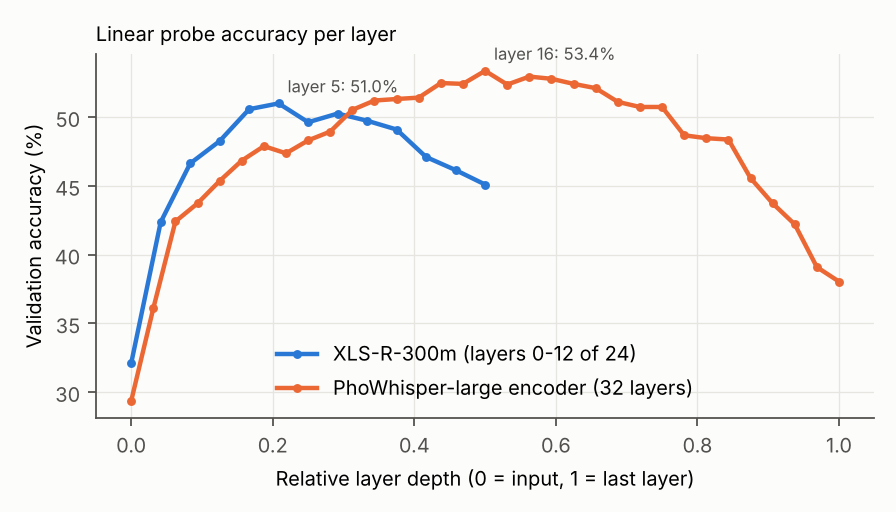
\includegraphics[width=\columnwidth]{figs/en_fig_layers.png}
\caption{Linear-probe validation accuracy for each layer, plotted against relative depth. Only layers 0 to 12 of XLS-R were extracted.}
\label{fig:layers}
\end{figure}

\subsection{Errors Follow Geography}
When the model is wrong, it is usually wrong nearby. For the first XLS-R baseline, wrong predictions were on average 267\,km from the true province, against 682\,km for a random wrong guess. In the final model, the number of confusions between two provinces falls with their distance (Spearman $\rho = -0.33$, $p < 10^{-90}$), and 76\% of all test utterances are placed within 100\,km of the true province. Accent varies continuously across the country, and the model's errors reflect that even with plain cross-entropy; Geo-LS strengthens it.

\subsection{Easy and Hard Provinces}
Per-province accuracy ranges from 6\% to 100\% (Fig.~\ref{fig:map}). The hardest provinces are \vn{Bạc Liêu} (6\%), \vn{Trà Vinh} (13\%), \vn{Lai Châu} (19\%), \vn{Đắk Nông} (26\%) and \vn{Điện Biên} (29\%); \vn{Bắc Giang}, \vn{Bình Định} and \vn{Kon Tum} reach 100\%. A plausible reading is that the hard provinces sound very close to their neighbours in the Mekong Delta, or have mixed migrant populations in the highlands; we have not verified this. Some of the easiest provinces, such as \vn{Ninh Bình}, also have a distinctive recording channel, so their scores may be partly inflated.

\begin{figure}[t]
\centering
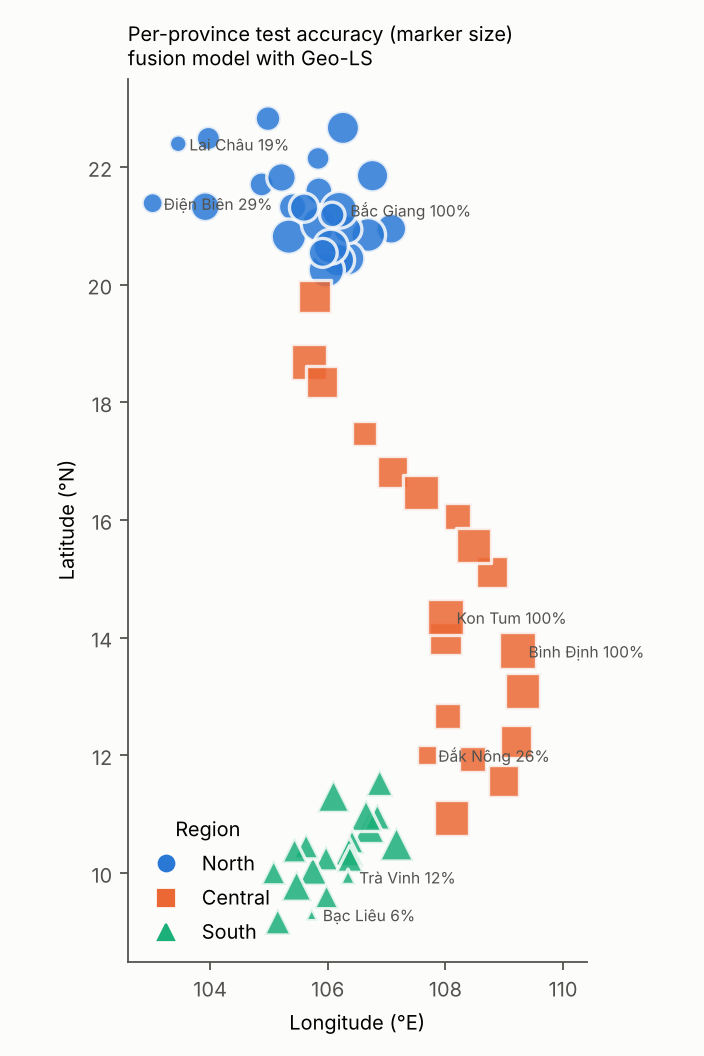
\includegraphics[width=0.78\columnwidth]{figs/en_fig_map.png}
\caption{Per-province test accuracy of the fusion model with Geo-LS. Each marker sits at the province capital; its size is proportional to accuracy.}
\label{fig:map}
\end{figure}

%======================================================================
\section{Limitations}
\textit{Recording channel.} Province labels are partly confounded with recording conditions. Our controls show that most accuracy survives when channel and content cues fail, but they cannot remove the confound entirely. Reported accuracy should be read as accuracy on ViMD-like recordings, not on arbitrary microphones.

\textit{No out-of-domain test.} All results come from the ViMD test split. We have not evaluated on independently collected recordings, such as phone speech from known speakers, where we expect a substantial drop.

\textit{Small data per class.} With about 240 training utterances per province, fine-tuning and larger heads overfit. Our negative fine-tuning results hold for the configurations we tried (two schedules), not for fine-tuning in general; parameter-efficient methods such as LoRA or adapters remain untested.

\textit{Approximate geography.} Each province is reduced to the coordinates of its capital, and labels follow the 63-province boundaries in force before the 2025 merger. Speakers may not live in, or speak like, the capital region.

\textit{Validation--test gap.} Validation accuracy is about 6 points above test accuracy for every model, so comparisons between models are consistent, but absolute validation numbers are optimistic. We draw conclusions from test results only.

\textit{Comparison with prior work.} The ViMD baselines use a different protocol (fine-tuning, 10-second segments), so the gain over them combines several factors.

%======================================================================
\section{Conclusion}
Frozen self-supervised encoders with a learned layer-weighted head identify the province of a Vietnamese speaker with 63.9\% accuracy using a single fused XLS-R and PhoWhisper model, and 64.6\% with an ensemble, on the 63-province ViMD test set, well above the 0.411 macro-F1 published with the dataset. Controls with transcripts, long-term spectra and place-name-free subsets indicate that most of this accuracy reflects accent rather than spoken content or recording channel. Geo-aware Label Smoothing reduces the geographic error of every model we tried by 8 to 19\,km against standard label smoothing, and on the strongest model it does so at no measurable cost in accuracy. In this low-resource regime, changing the training target was more effective than full fine-tuning, LP-FT or temporal CNN and Transformer heads.

Three directions follow. First, testing on independently recorded speech would measure how far the system generalises beyond ViMD's recording conditions. Second, adversarial training against speaker or channel information could reduce the remaining confound. Third, parameter-efficient fine-tuning, and joint dialect identification and speech recognition using ViMD's transcripts, could show whether adaptation helps once overfitting is controlled.

%======================================================================
\begin{thebibliography}{99}

\bibitem{vimd}
N. Van Dinh, T. C. Dang, L. T. Nguyen, and K. Van Nguyen, ``Multi-dialect Vietnamese: Task, dataset, baseline models and challenges,'' in \textit{Proc. EMNLP}, 2024, arXiv:2410.03458.

\bibitem{wav2vec2}
A. Baevski, H. Zhou, A. Mohamed, and M. Auli, ``wav2vec 2.0: A framework for self-supervised learning of speech representations,'' in \textit{Proc. NeurIPS}, 2020.

\bibitem{xlsr}
A. Babu, C. Wang, A. Tjandra \textit{et al.}, ``XLS-R: Self-supervised cross-lingual speech representation learning at scale,'' in \textit{Proc. Interspeech}, 2022.

\bibitem{whisper}
A. Radford, J. W. Kim, T. Xu, G. Brockman, C. McLeavey, and I. Sutskever, ``Robust speech recognition via large-scale weak supervision,'' in \textit{Proc. ICML}, 2023.

\bibitem{phowhisper}
T.-T. Le, L. T. Nguyen, and D. Q. Nguyen, ``PhoWhisper: Automatic speech recognition for Vietnamese,'' in \textit{Proc. ICLR Tiny Papers}, 2024.

\bibitem{superb}
S. Yang, P.-H. Chi, Y.-S. Chuang \textit{et al.}, ``SUPERB: Speech processing universal performance benchmark,'' in \textit{Proc. Interspeech}, 2021.

\bibitem{pasad}
A. Pasad, J.-C. Chou, and K. Livescu, ``Layer-wise analysis of a self-supervised speech representation model,'' in \textit{Proc. IEEE ASRU}, 2021.

\bibitem{asp}
K. Okabe, T. Koshinaka, and K. Shinoda, ``Attentive statistics pooling for deep speaker embedding,'' in \textit{Proc. Interspeech}, 2018.

\bibitem{ecapa}
B. Desplanques, J. Thienpondt, and K. Demuynck, ``ECAPA-TDNN: Emphasized channel attention, propagation and aggregation in TDNN based speaker verification,'' in \textit{Proc. Interspeech}, 2020.

\bibitem{lpft}
A. Kumar, A. Raghunathan, R. Jones, T. Ma, and P. Liang, ``Fine-tuning can distort pretrained features and underperform out-of-distribution,'' in \textit{Proc. ICLR}, 2022.

\bibitem{inception}
C. Szegedy, V. Vanhoucke, S. Ioffe, J. Shlens, and Z. Wojna, ``Rethinking the Inception architecture for computer vision,'' in \textit{Proc. IEEE CVPR}, 2016.

\bibitem{muller}
R. M\"uller, S. Kornblith, and G. Hinton, ``When does label smoothing help?'' in \textit{Proc. NeurIPS}, 2019.

\bibitem{sord}
R. D\'iaz and A. Marathe, ``Soft labels for ordinal regression,'' in \textit{Proc. IEEE CVPR}, 2019.

\bibitem{bettermistakes}
L. Bertinetto, R. Mueller, K. Tertikas, S. Samangooei, and N. A. Lord, ``Making better mistakes: Leveraging class hierarchies with deep networks,'' in \textit{Proc. IEEE CVPR}, 2020.

\bibitem{specaugment}
D. S. Park, W. Chan, Y. Zhang \textit{et al.}, ``SpecAugment: A simple data augmentation method for automatic speech recognition,'' in \textit{Proc. Interspeech}, 2019.

\bibitem{phobert}
D. Q. Nguyen and A. T. Nguyen, ``PhoBERT: Pre-trained language models for Vietnamese,'' in \textit{Findings of EMNLP}, 2020.

\end{thebibliography}

\end{document}
